

\section{Dataset}
We have collected several sequences with the sensor rig to showcase the potential of the system.
The current dataset consists of one sequence where we filmed a moving \gls{usv} from land, one where we recorded data from a moving ship driving in the city canal and a two scenes where we walk along the river and film the water surface from different angles.
The dataset contains the raw data from the cameras together with metadata for each frame, raw data from the \gls{imu} and raw data from the \gls{gnss} receivers.
As we want to ensure quality before releasing calibration data, we currently provide a calibration sequence where we film a chess board while rotating the sensor rig, which can be used for calibration purposes.
A representative selection of images from the dataset can be found at the end of the paper, where we show the $S0$ image on the left and the polarized image or unpolaraized image on the right.

The dataset is available at \url{https://github.com/emillma/datasets}.

\section{Conclusion and Future Work}
In this paper we have presented a new portable sensor rig which makes collecting sensor data in maritime environments significantly easier.
The platform is self-contained, and its ease of use has already allowed multiple researchers to use it for their data collection.
With the two polarization cameras currently mounted on the sensor rig, we have collected several video sequences that strongly indicate the benefint of using color polarization cameras in the maritime domain.

While we have synchronized the sensors, accurately estimating the extrinsic parameters remains to be done.
We intend to continue collecting and share more data collected from the shore as well as moving vessels of different sizes, under different weather conditions and at different times of the day.

TODO add more future work and improve the conclusion.



\begin{figure}[H]
    \begin{subfigure}[T]{.49\textwidth}
        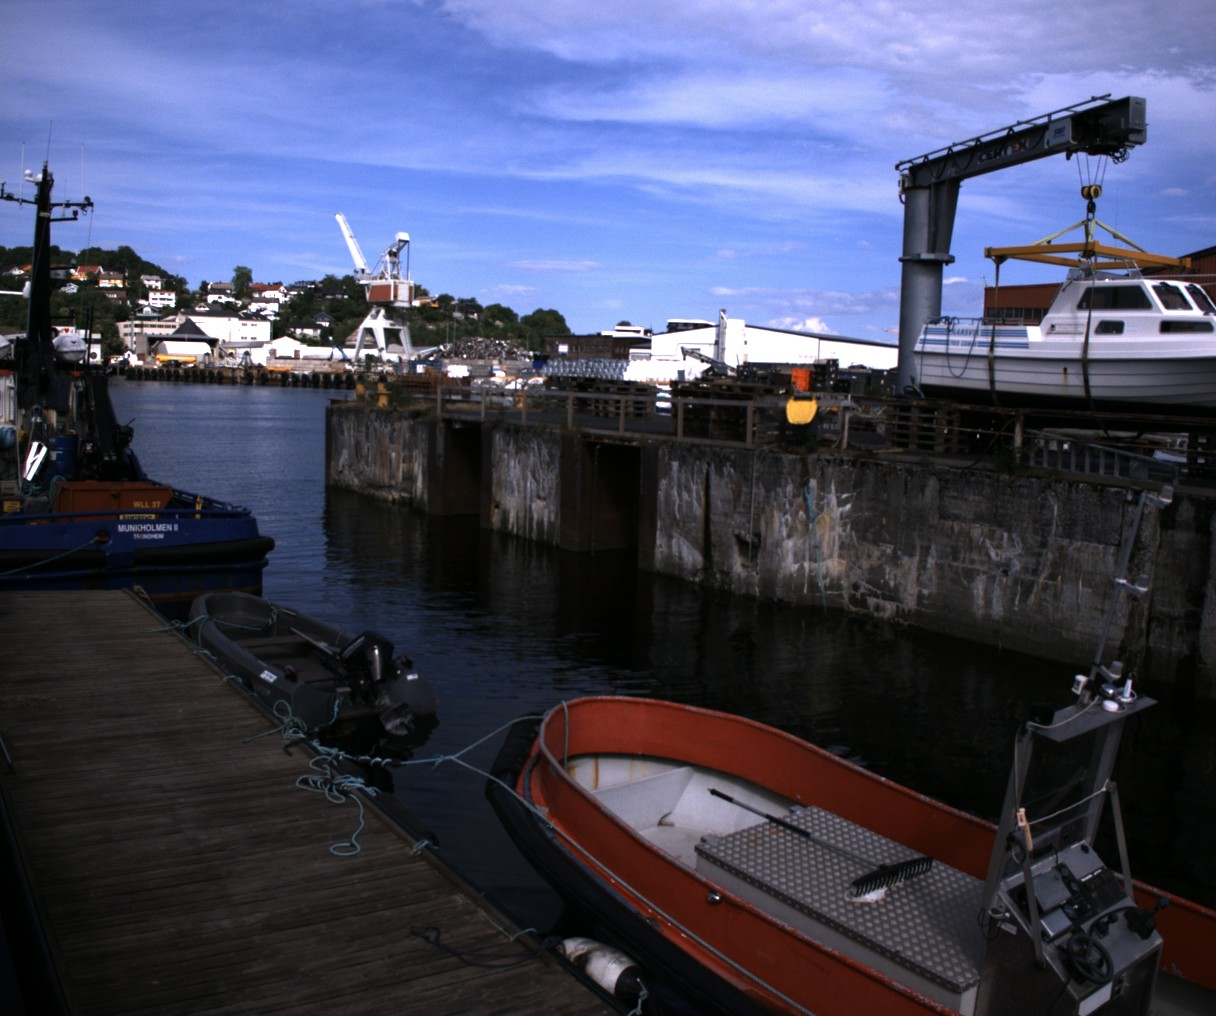
\includegraphics[width=\textwidth]{figures/pictures/img_2790_s0.jpg}
    \end{subfigure} \hfill
    \begin{subfigure}[T]{.49\textwidth}
        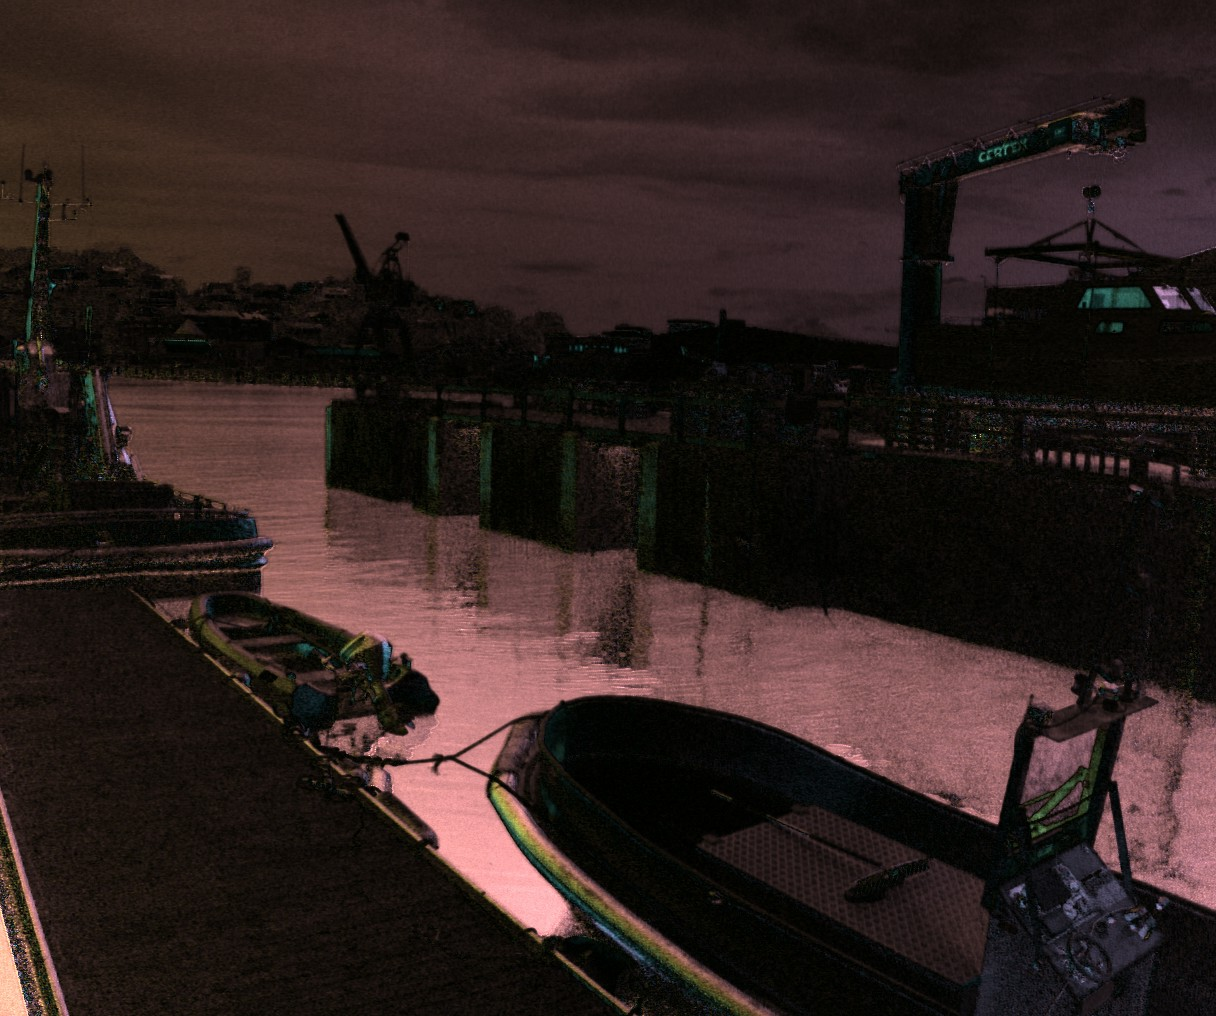
\includegraphics[width=\textwidth]{figures/pictures/img_2790_pol.jpg}
    \end{subfigure}
    \caption{Docking area.}
\end{figure}
\vspace{-.5cm}

\begin{figure}[H]
    \begin{subfigure}[T]{.49\textwidth}
        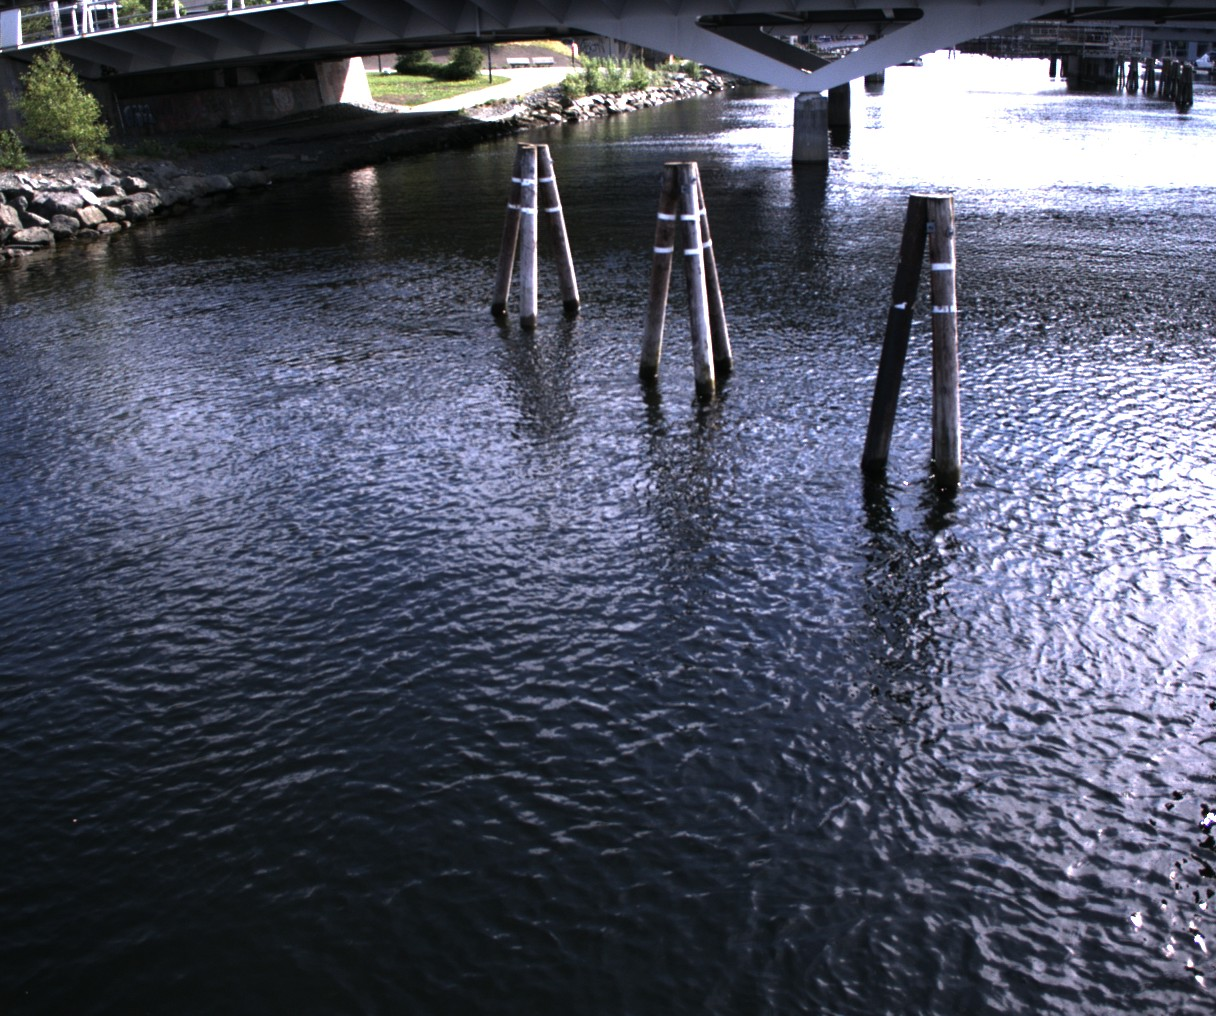
\includegraphics[width=\textwidth]{figures/pictures/img_7458_s0.jpg}
    \end{subfigure} \hfill
    \begin{subfigure}[T]{.49\textwidth}
        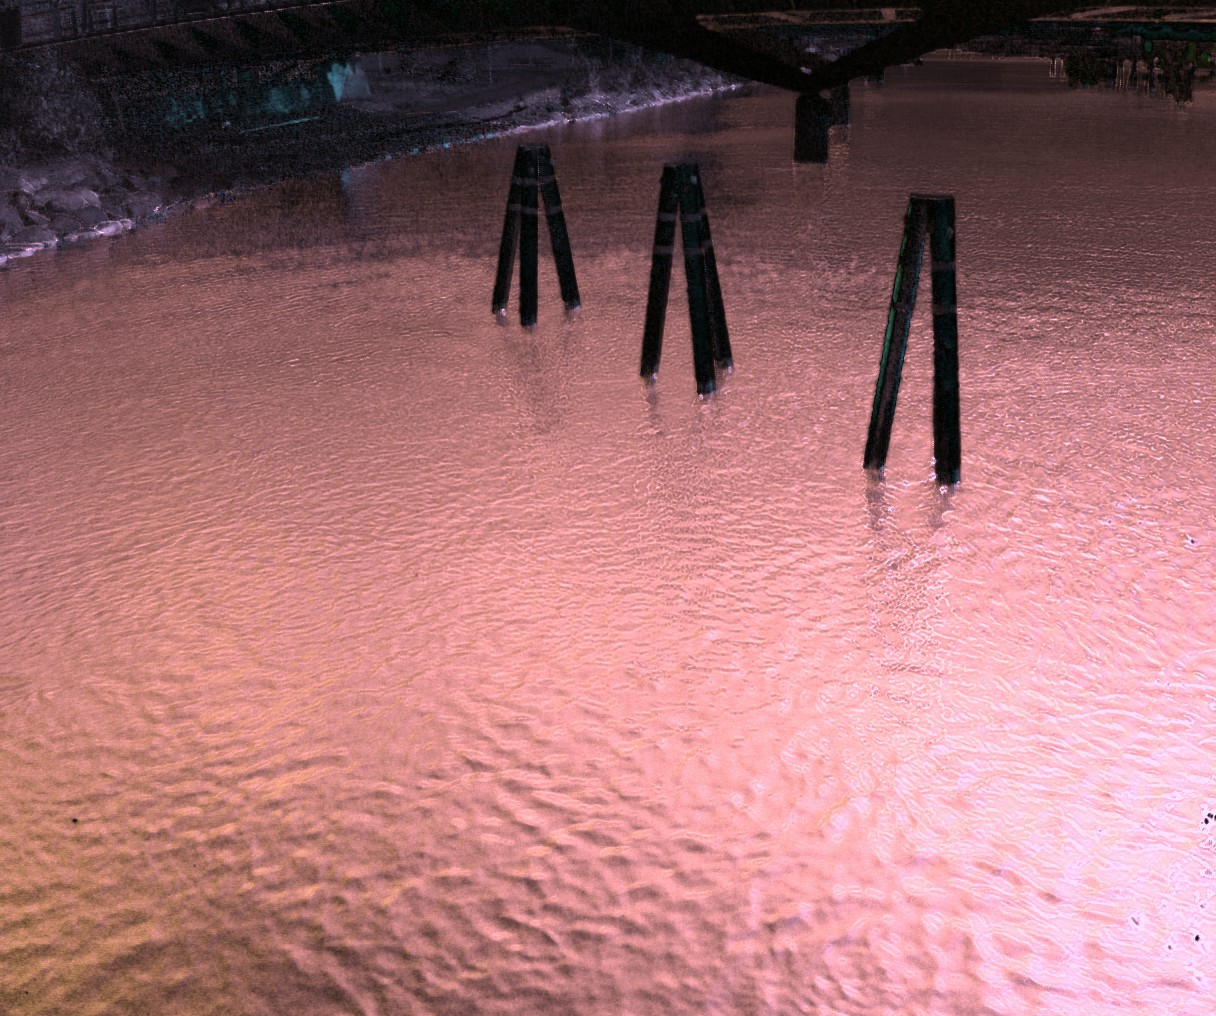
\includegraphics[width=\textwidth]{figures/pictures/img_7458_pol.jpg}
        
    \end{subfigure}
    \caption{Wooden posts in the water.}
\end{figure}
\vspace{-.5cm}

\begin{figure}[H]
    \begin{subfigure}[T]{.49\textwidth}
        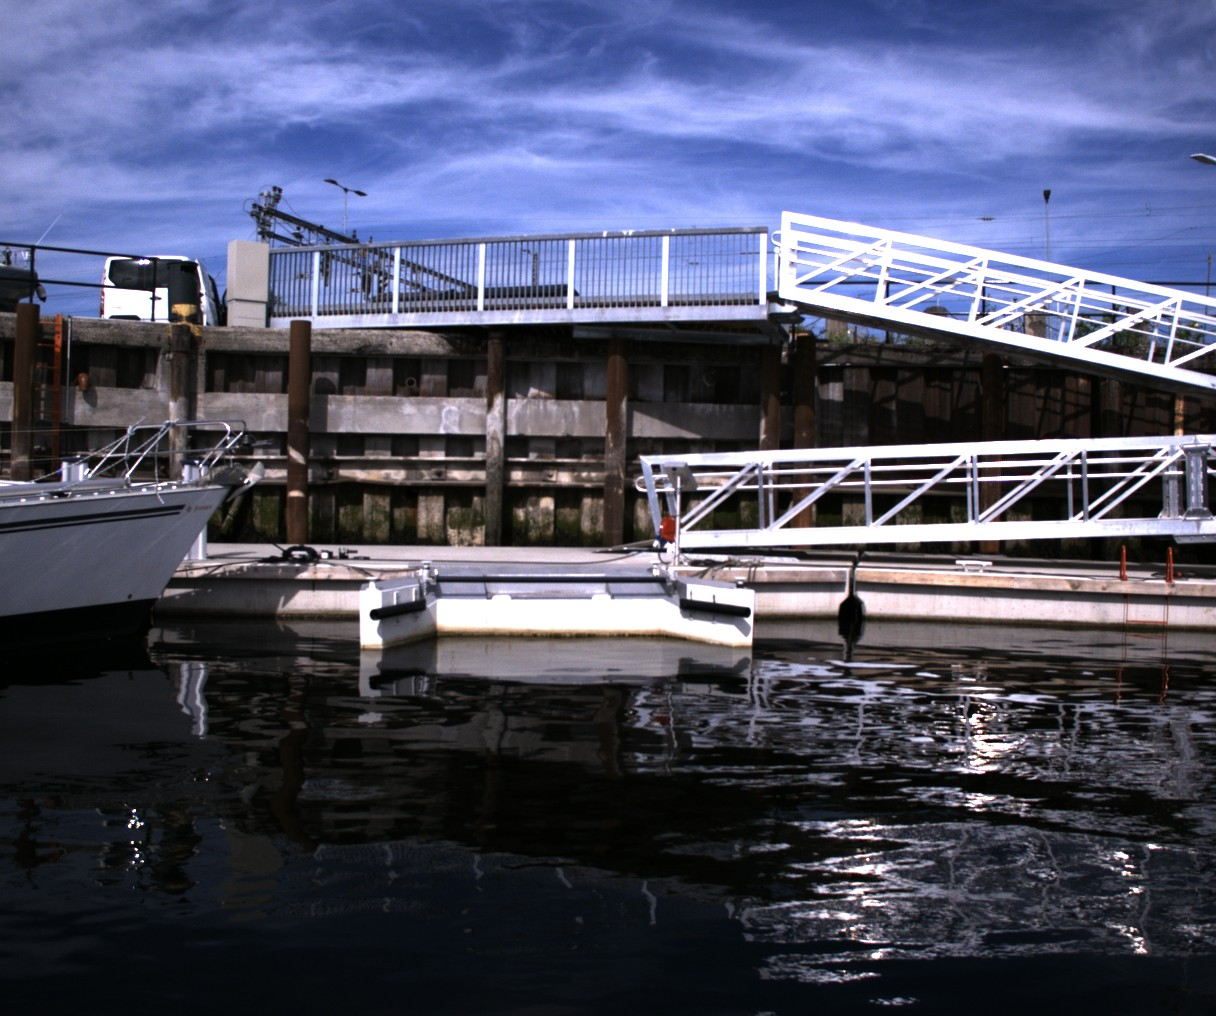
\includegraphics[width=\textwidth]{figures/pictures/img_11640_s0.jpg}
    \end{subfigure} \hfill
    \begin{subfigure}[T]{.49\textwidth}
        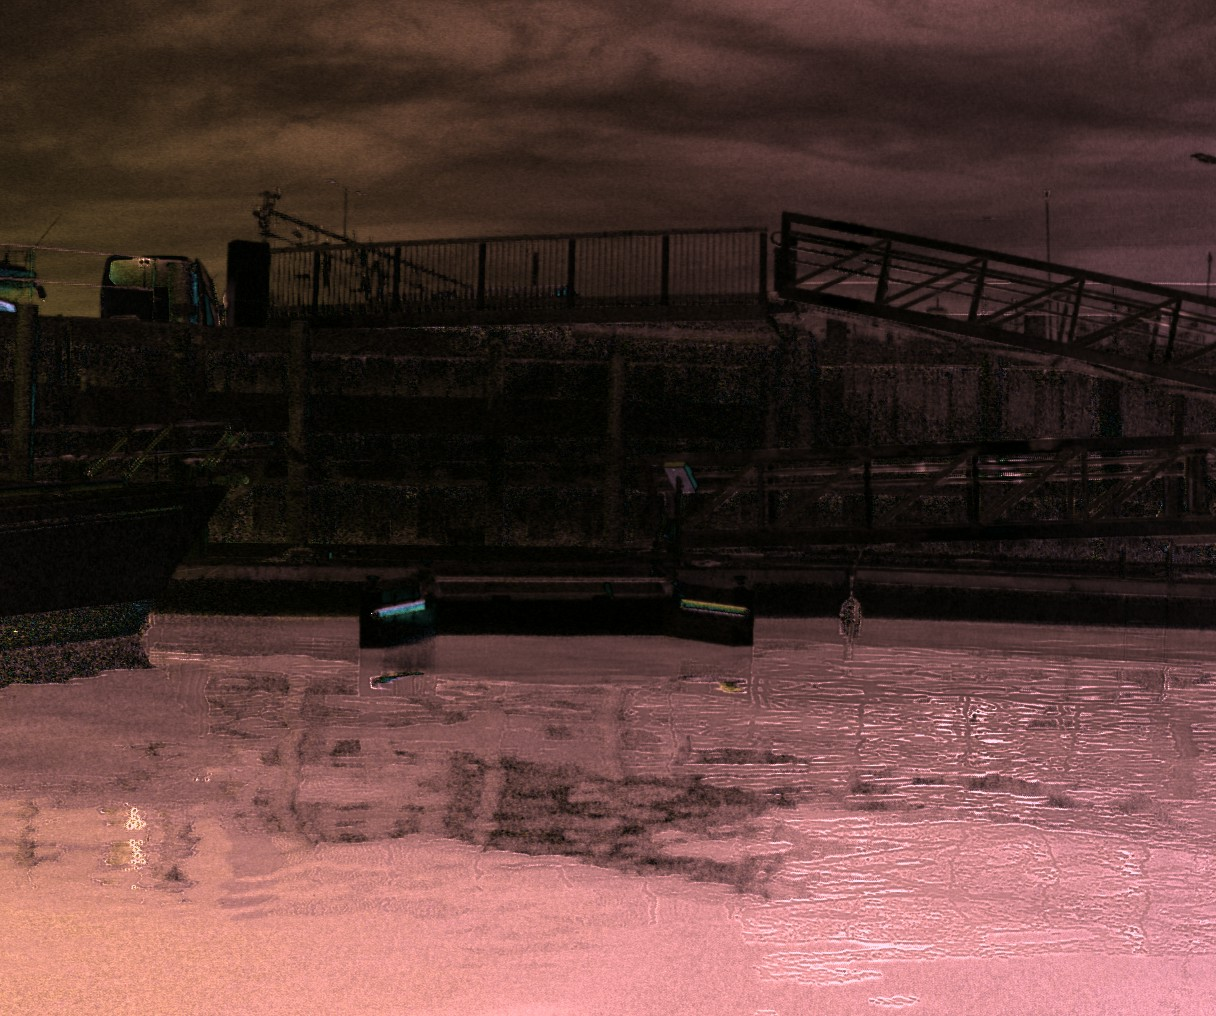
\includegraphics[width=\textwidth]{figures/pictures/img_11640_pol.jpg}
    \end{subfigure}
    \caption{Dock viewed from the water.}
\end{figure}
\vspace{-.5cm}

\begin{figure}[H]
    \begin{subfigure}[T]{.49\textwidth}
        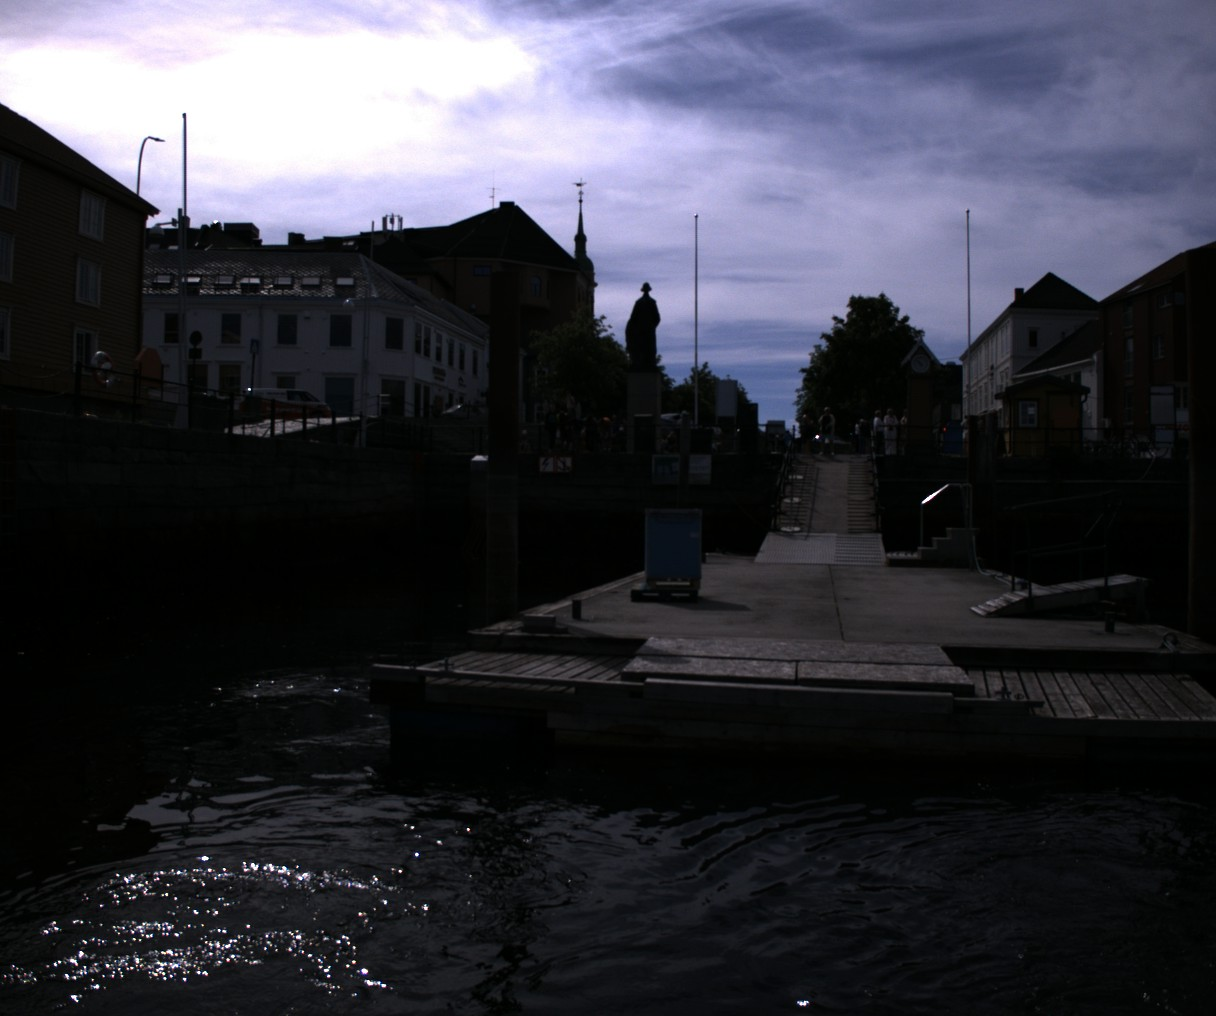
\includegraphics[width=\textwidth]{figures/pictures/img_10170_s0.jpg}
    \end{subfigure} \hfill
    \begin{subfigure}[T]{.49\textwidth}
        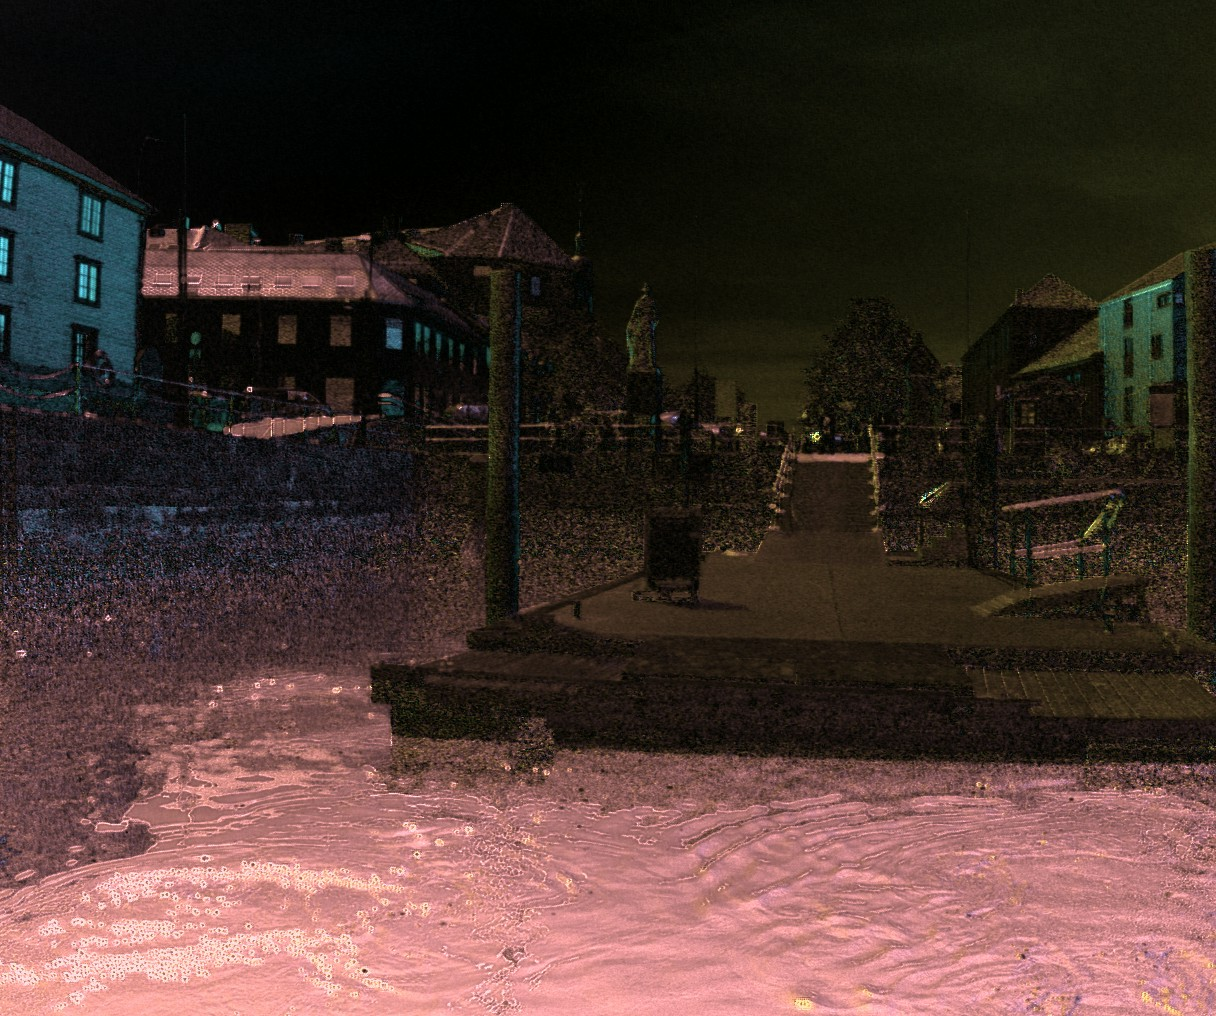
\includegraphics[width=\textwidth]{figures/pictures/img_10170_pol.jpg}
    \end{subfigure}
    \caption{Underexposed image of a dock seen from the water.}
\end{figure}
\vspace{-.5cm}


\begin{figure}[H]
    \begin{subfigure}[T]{.49\textwidth}
        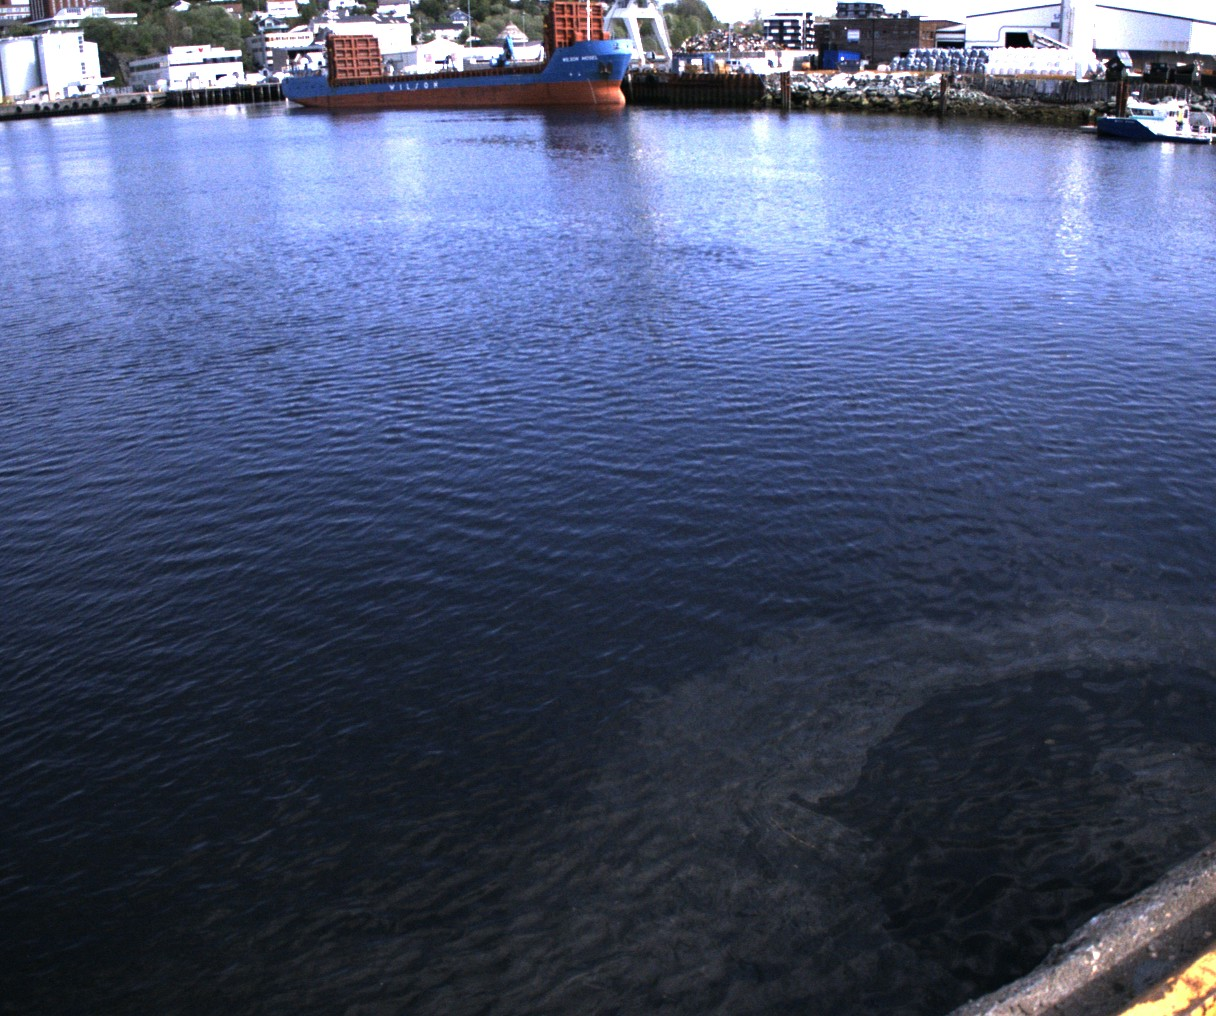
\includegraphics[width=\textwidth]{figures/pictures/img_3726_s0.jpg}
    \end{subfigure} \hfill
    \begin{subfigure}[T]{.49\textwidth}
        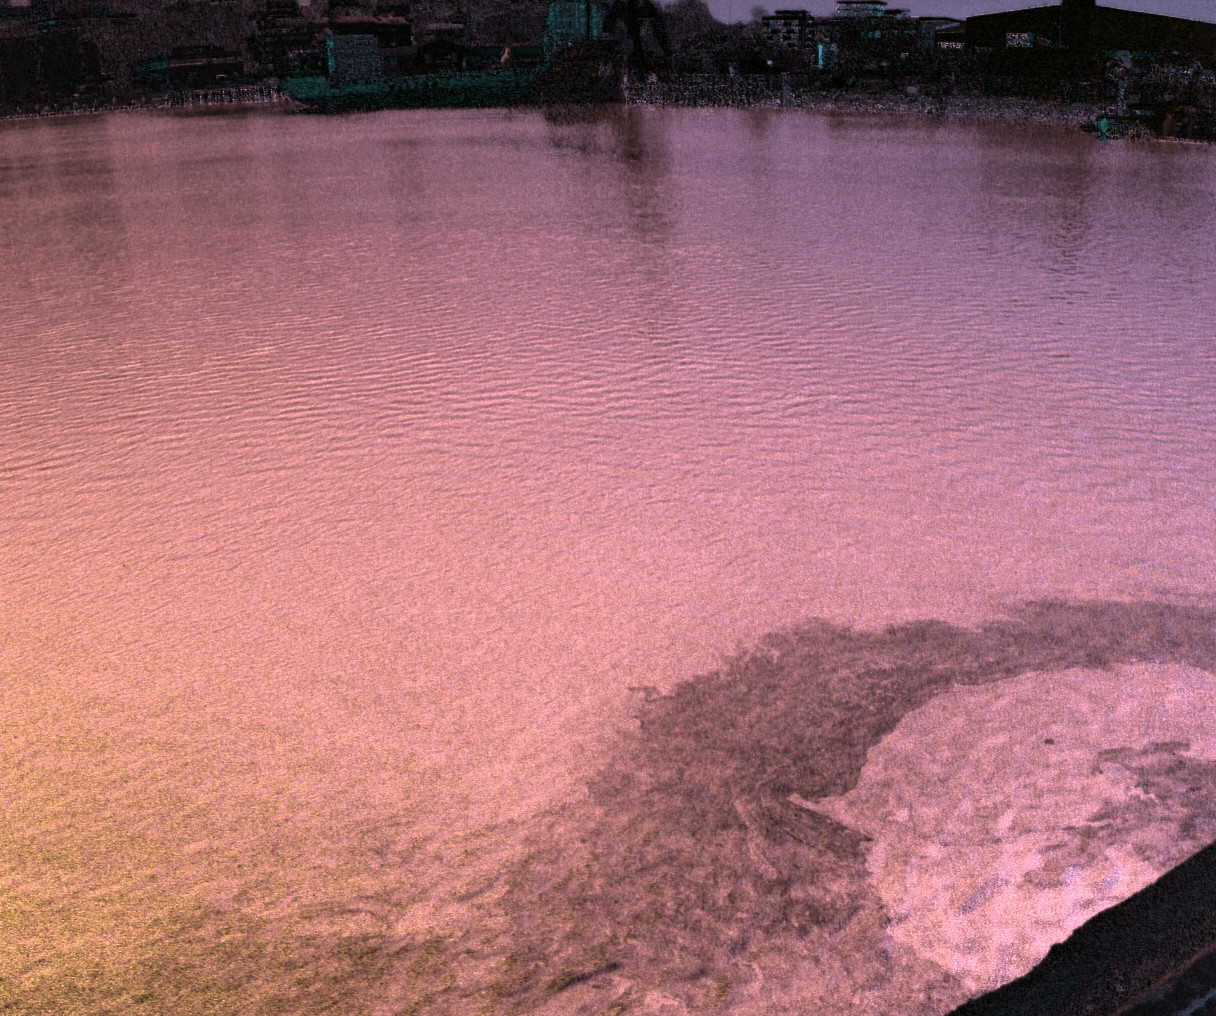
\includegraphics[width=\textwidth]{figures/pictures/img_3726_pol.jpg}
    \end{subfigure}
    \caption{Pollen on the water surface.}
\end{figure}
\vspace{-.5cm}

\begin{figure}[H]
    \begin{subfigure}[T]{.49\textwidth}
        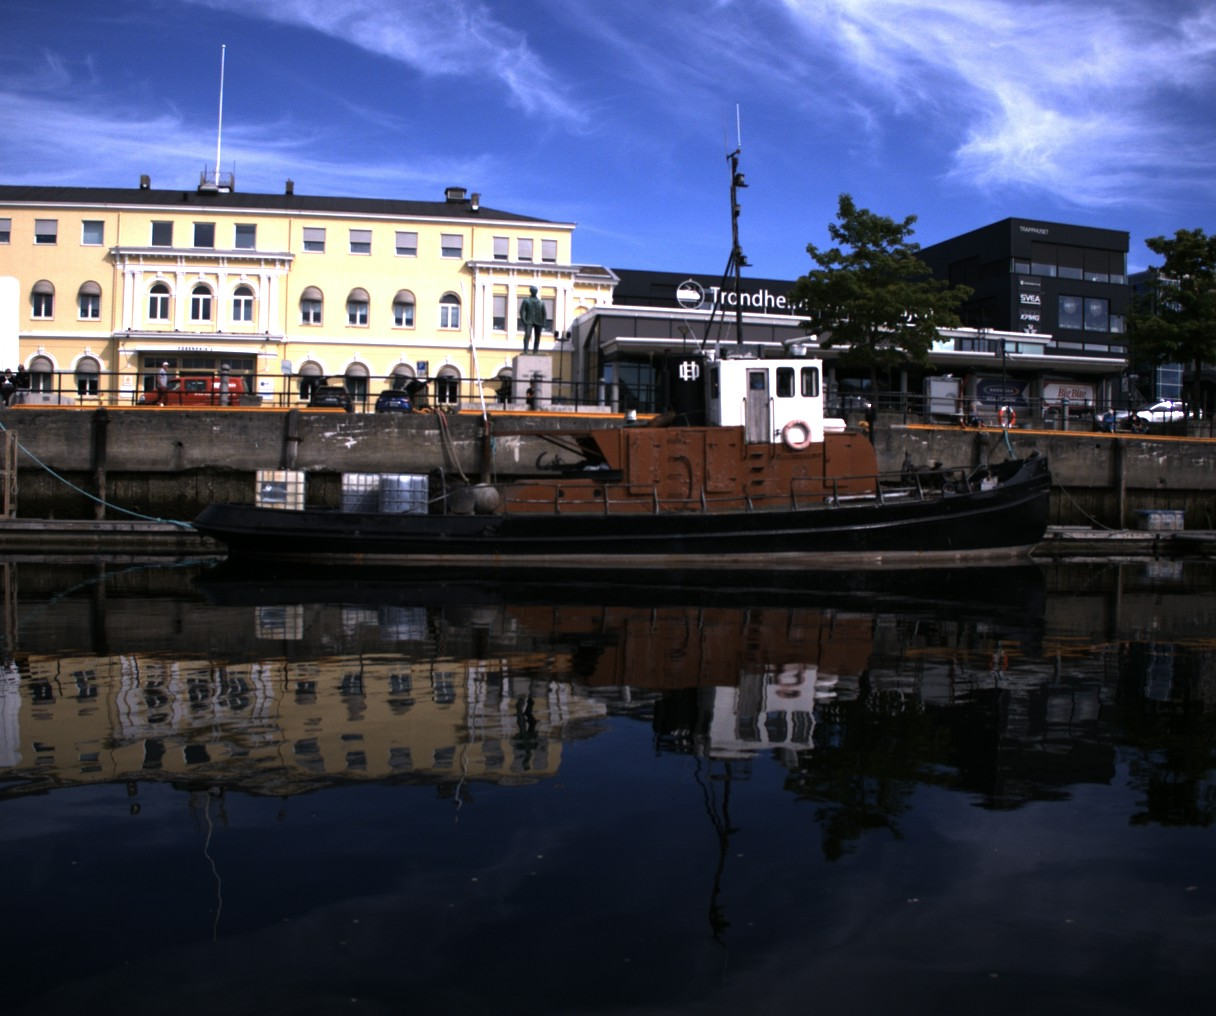
\includegraphics[width=\textwidth]{figures/pictures/img_4038_s0.jpg}
    \end{subfigure} \hfill
    \begin{subfigure}[T]{.49\textwidth}
        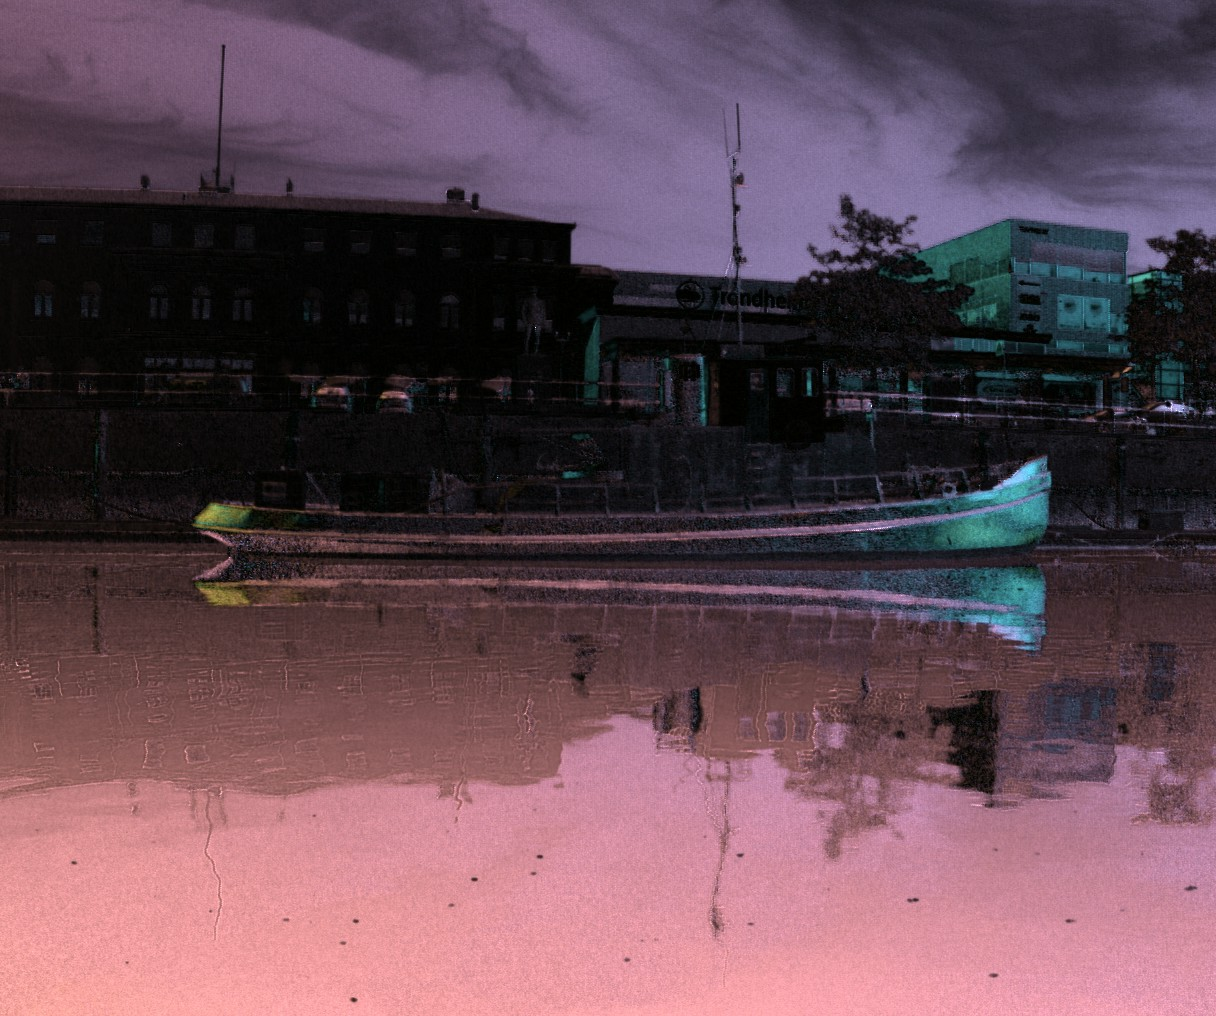
\includegraphics[width=\textwidth]{figures/pictures/img_4038_pol.jpg}
    \end{subfigure}
    \caption{A docked boat seen from the water.}
\end{figure}
\vspace{-.5cm}

% \begin{figure}[H]
%     \begin{subfigure}[T]{.49\textwidth}
%         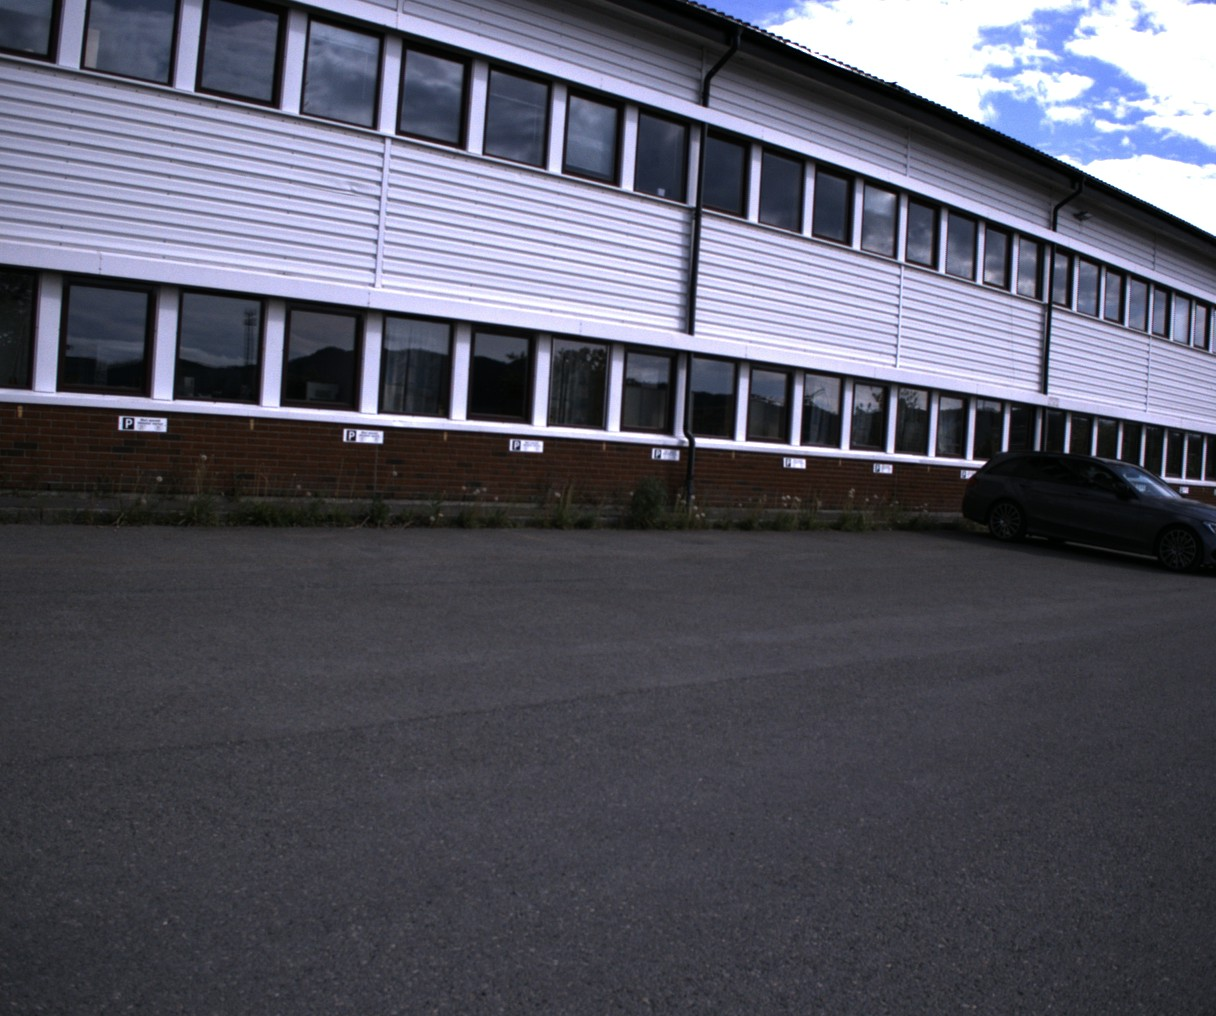
\includegraphics[width=\textwidth]{figures/pictures/img_5742_s0.jpg}
%     \end{subfigure} \hfill
%     \begin{subfigure}[T]{.49\textwidth}
%         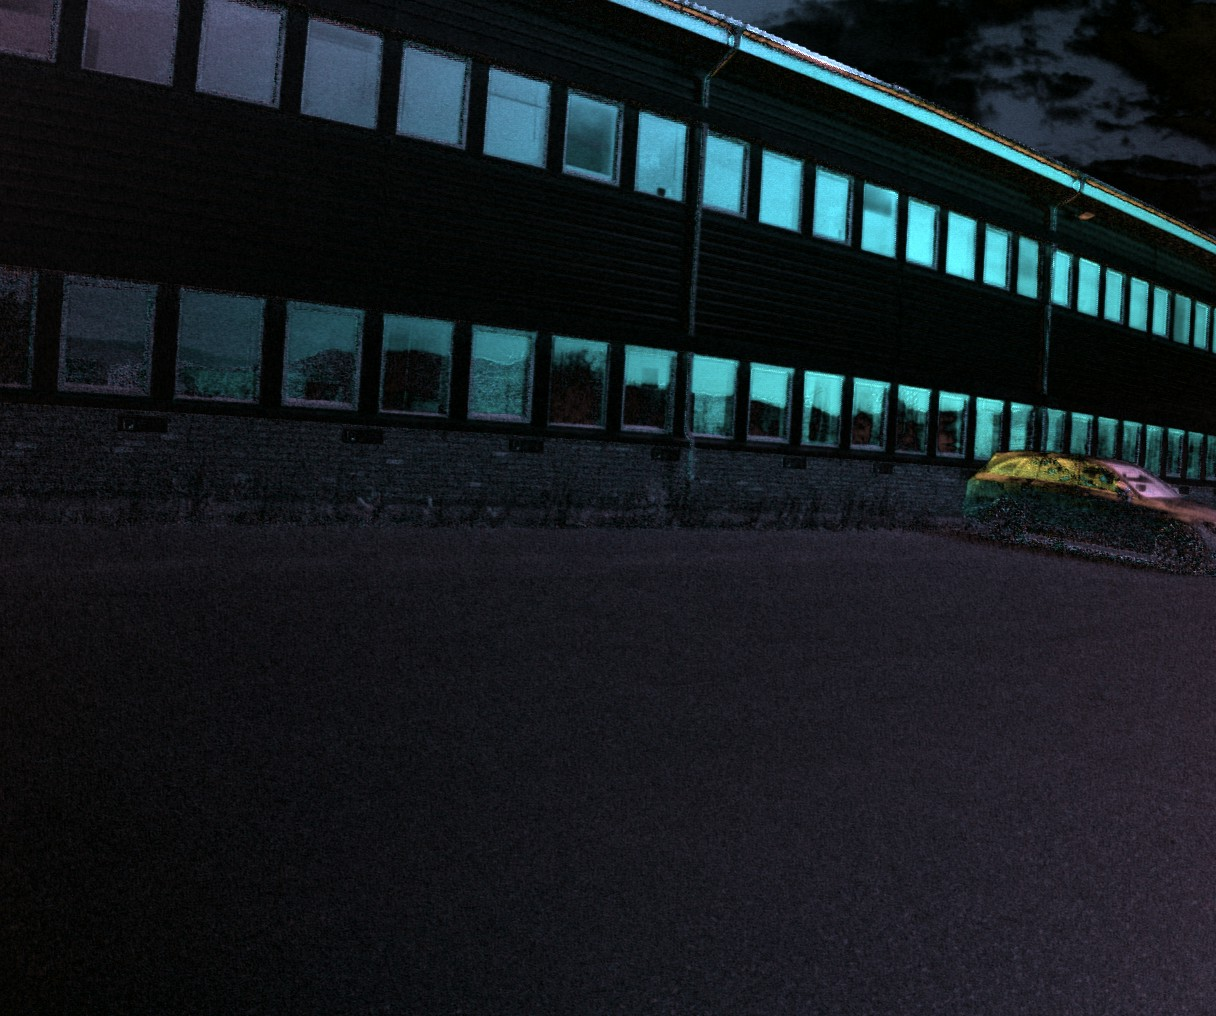
\includegraphics[width=\textwidth]{figures/pictures/img_5742_pol.jpg}
%     \end{subfigure}
%     \caption{Building with glass windows.}
% \end{figure}
% \vspace{-.5cm}
\begin{figure}[H]
    \begin{subfigure}[T]{.49\textwidth}
        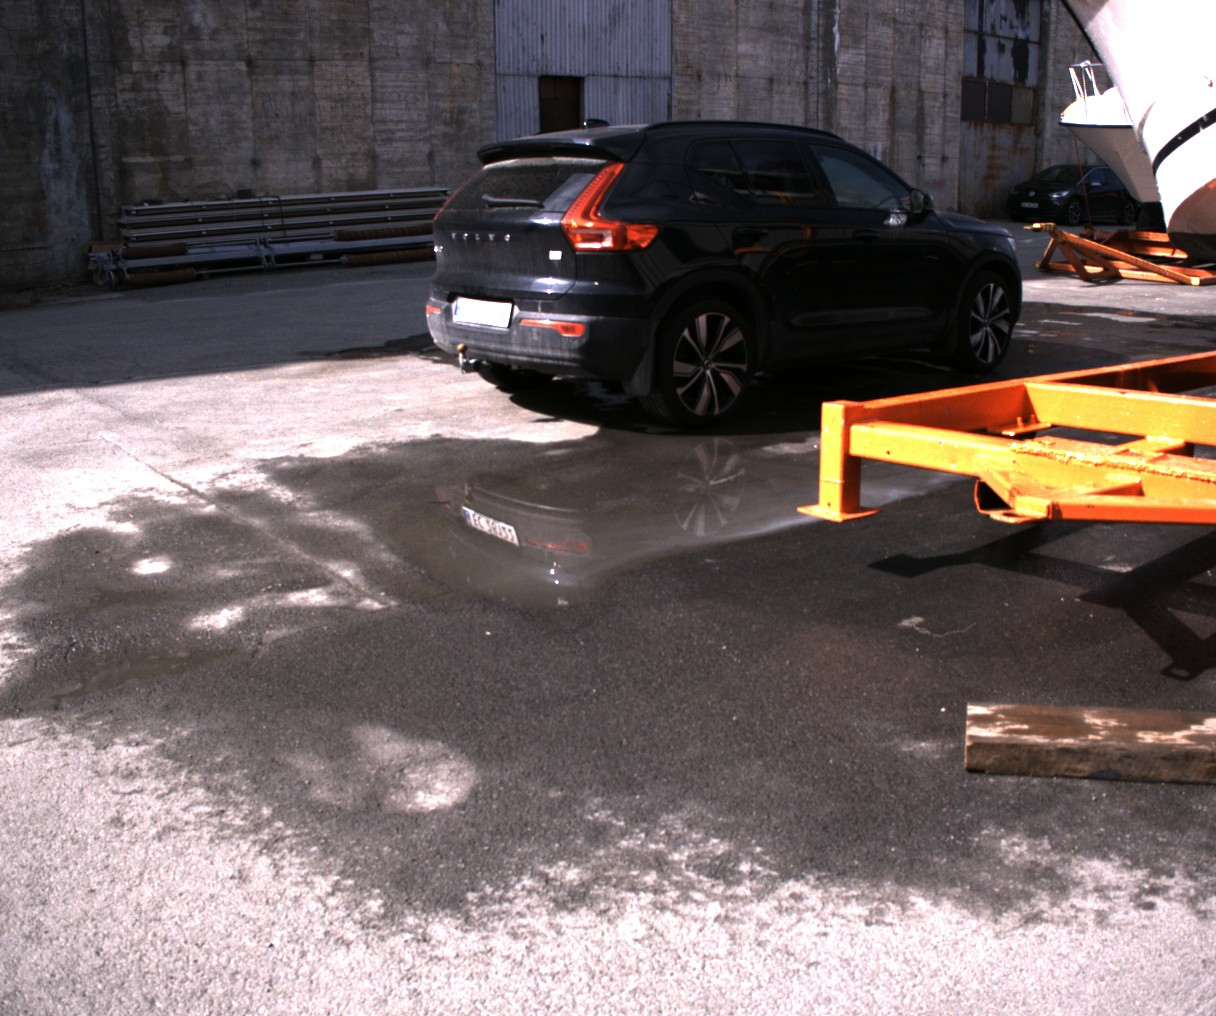
\includegraphics[width=\textwidth]{figures/pictures/img_1116_s0.jpg}
    \end{subfigure} \hfill
    \begin{subfigure}[T]{.49\textwidth}
        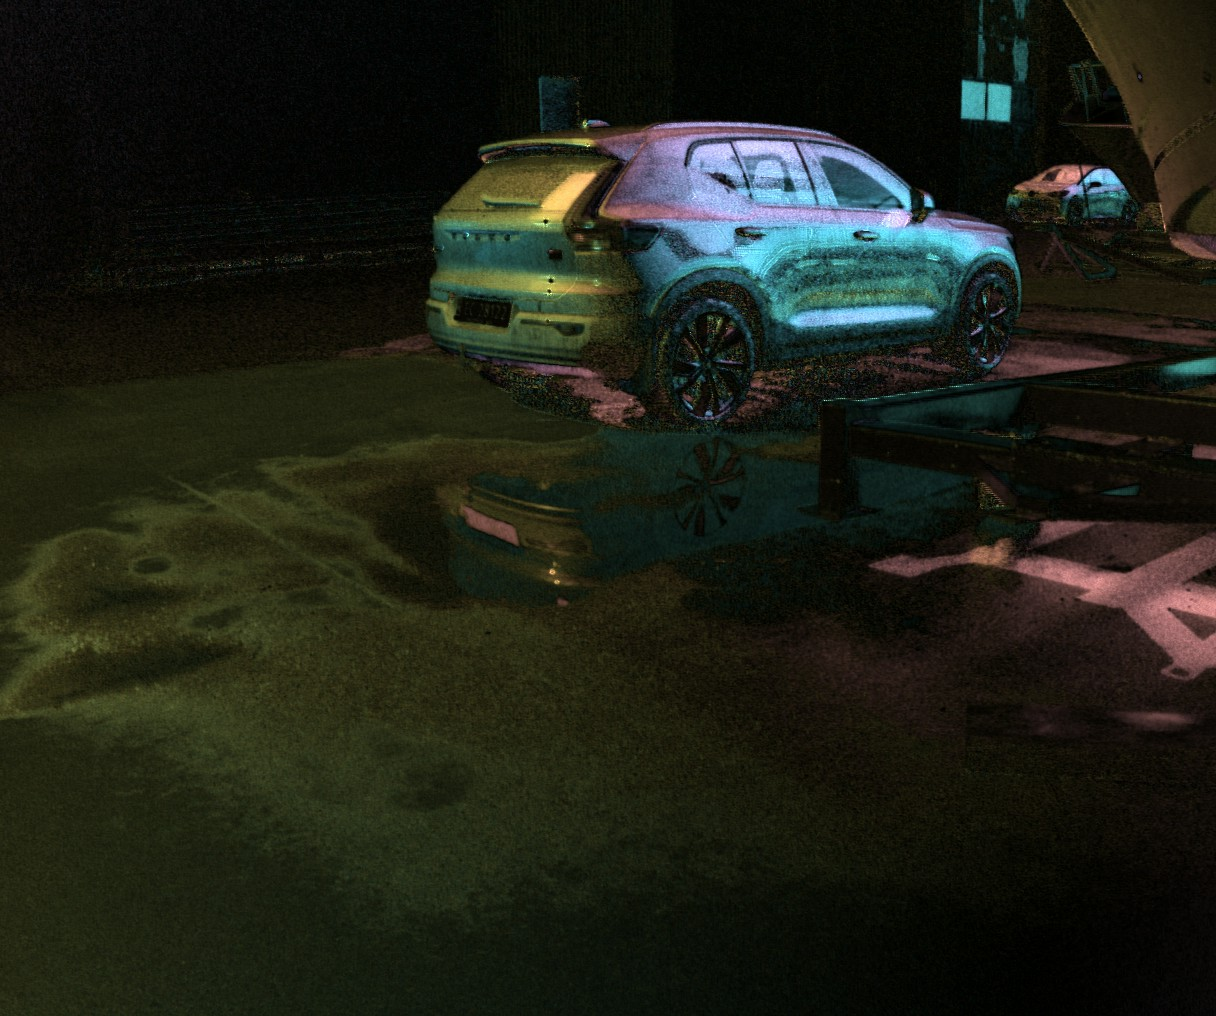
\includegraphics[width=\textwidth]{figures/pictures/img_1116_pol.jpg}
    \end{subfigure}
    \caption{A car standing next to a puddle of water.}
\end{figure}
\vspace{-.5cm}


\begin{figure}[H]
    \begin{subfigure}[T]{.49\textwidth}
        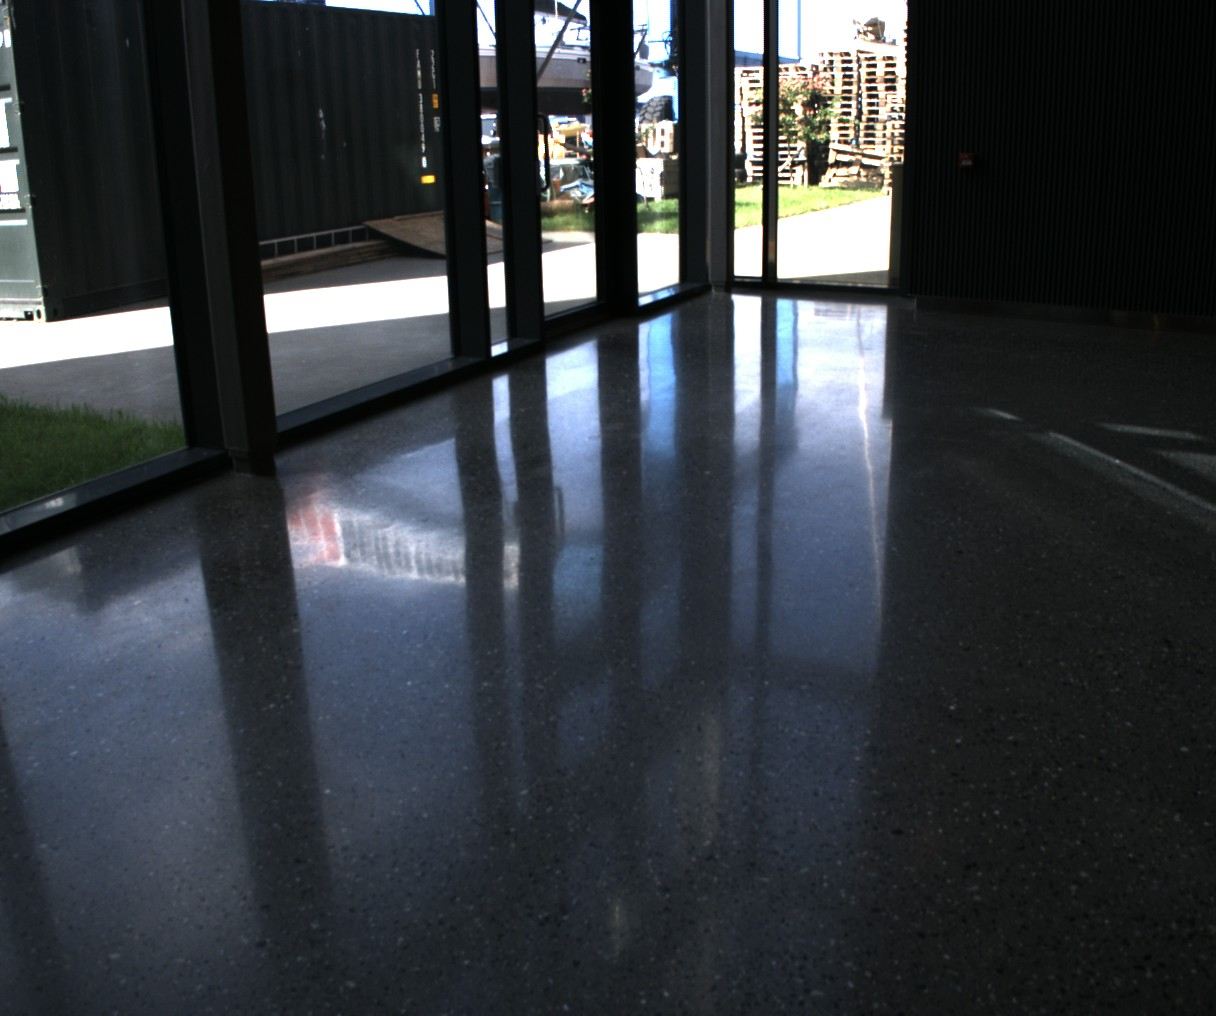
\includegraphics[width=\textwidth]{figures/pictures/img_9222_s0.jpg}
    \end{subfigure} \hfill
    \begin{subfigure}[T]{.49\textwidth}
        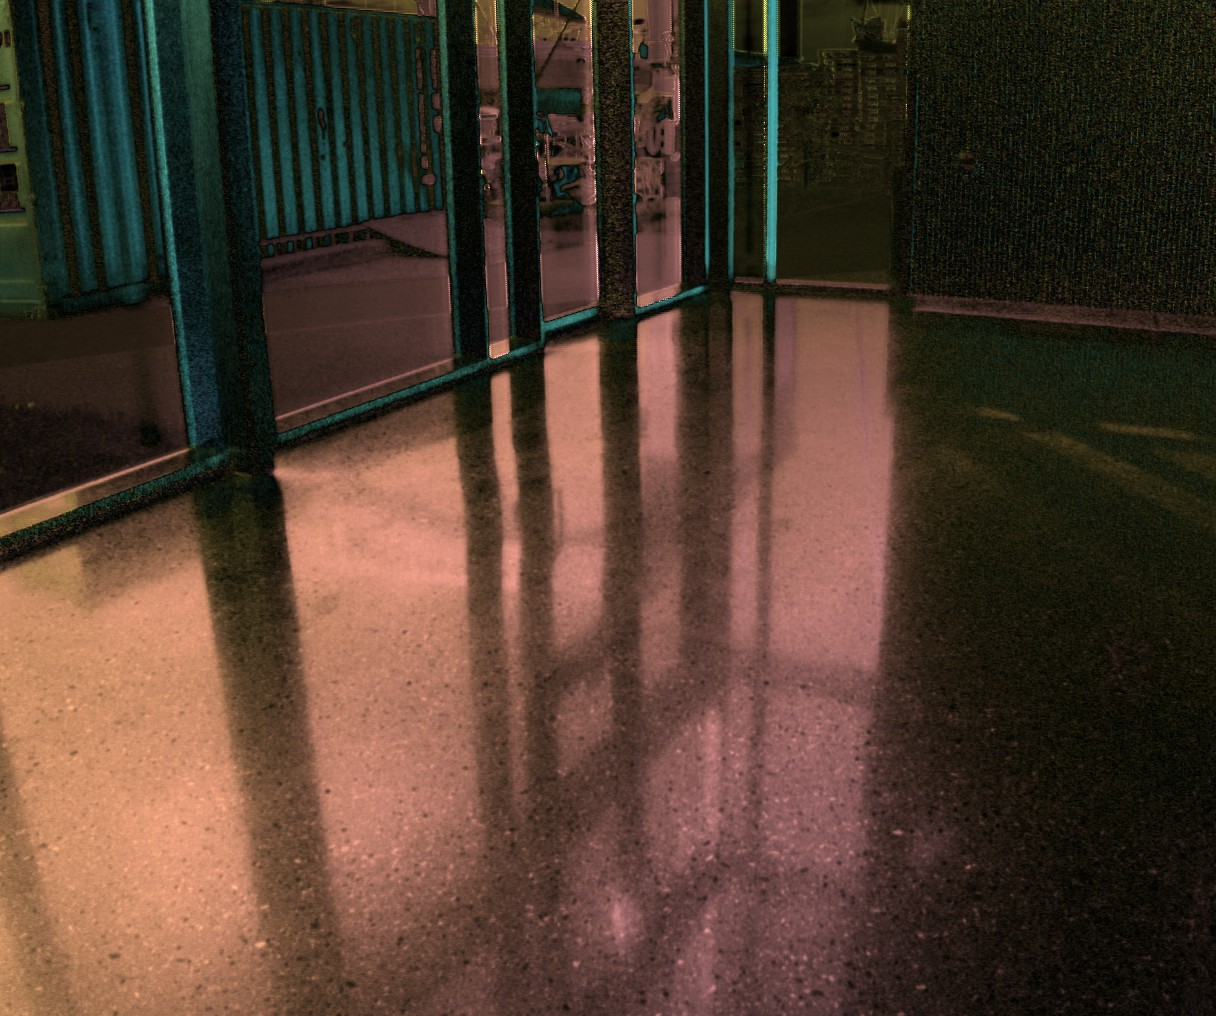
\includegraphics[width=\textwidth]{figures/pictures/img_9222_pol.jpg}
    \end{subfigure}
    \caption{Stone floor with reflections.}
\end{figure}
\vspace{-.5cm}

% \begin{figure}[H]
%     \begin{subfigure}[T]{.49\textwidth}
%         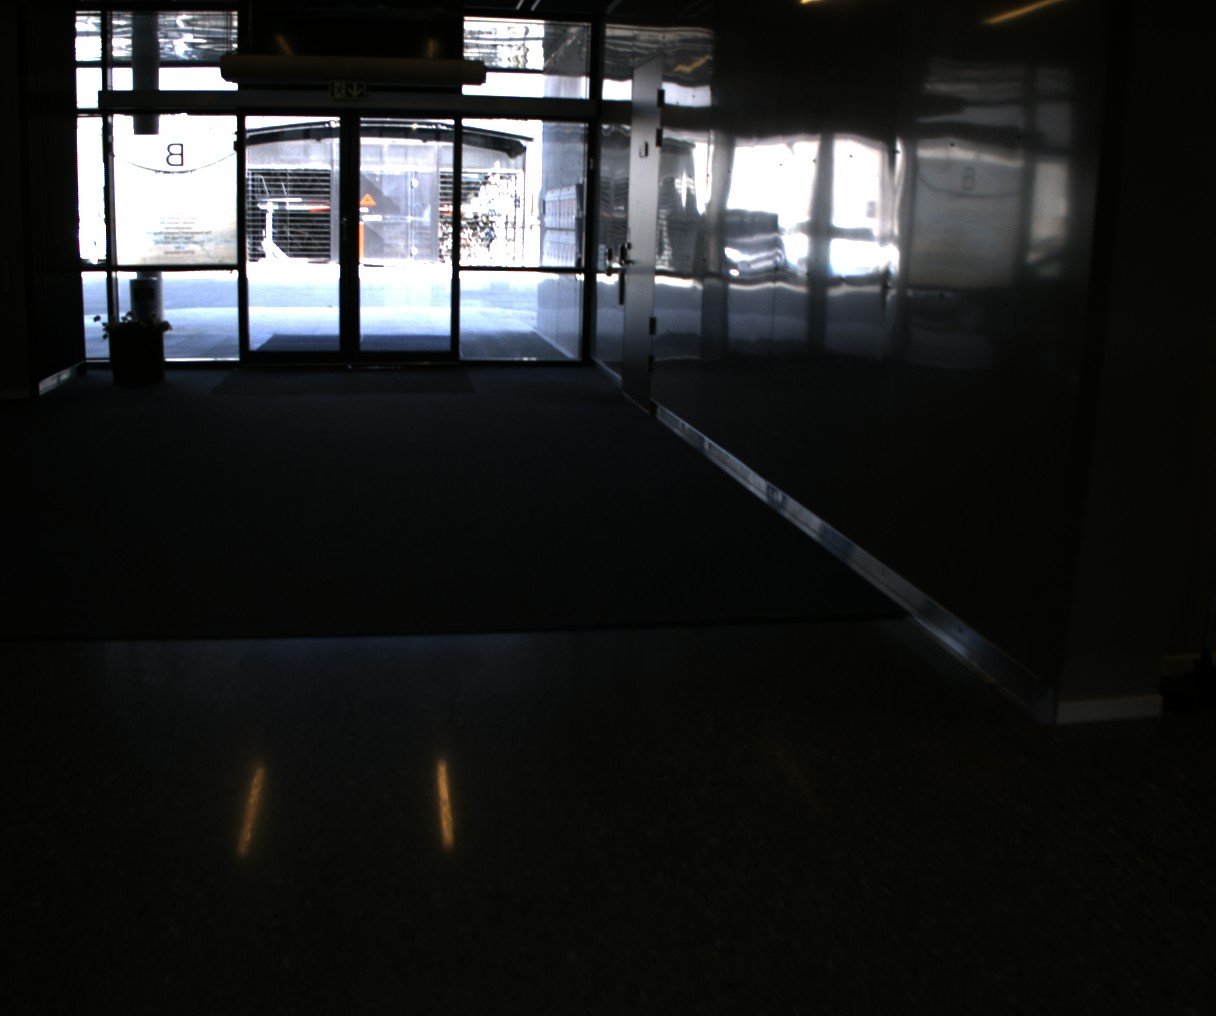
\includegraphics[width=\textwidth]{figures/pictures/img_9306_s0.jpg}
%     \end{subfigure} \hfill
%     \begin{subfigure}[T]{.49\textwidth}
%         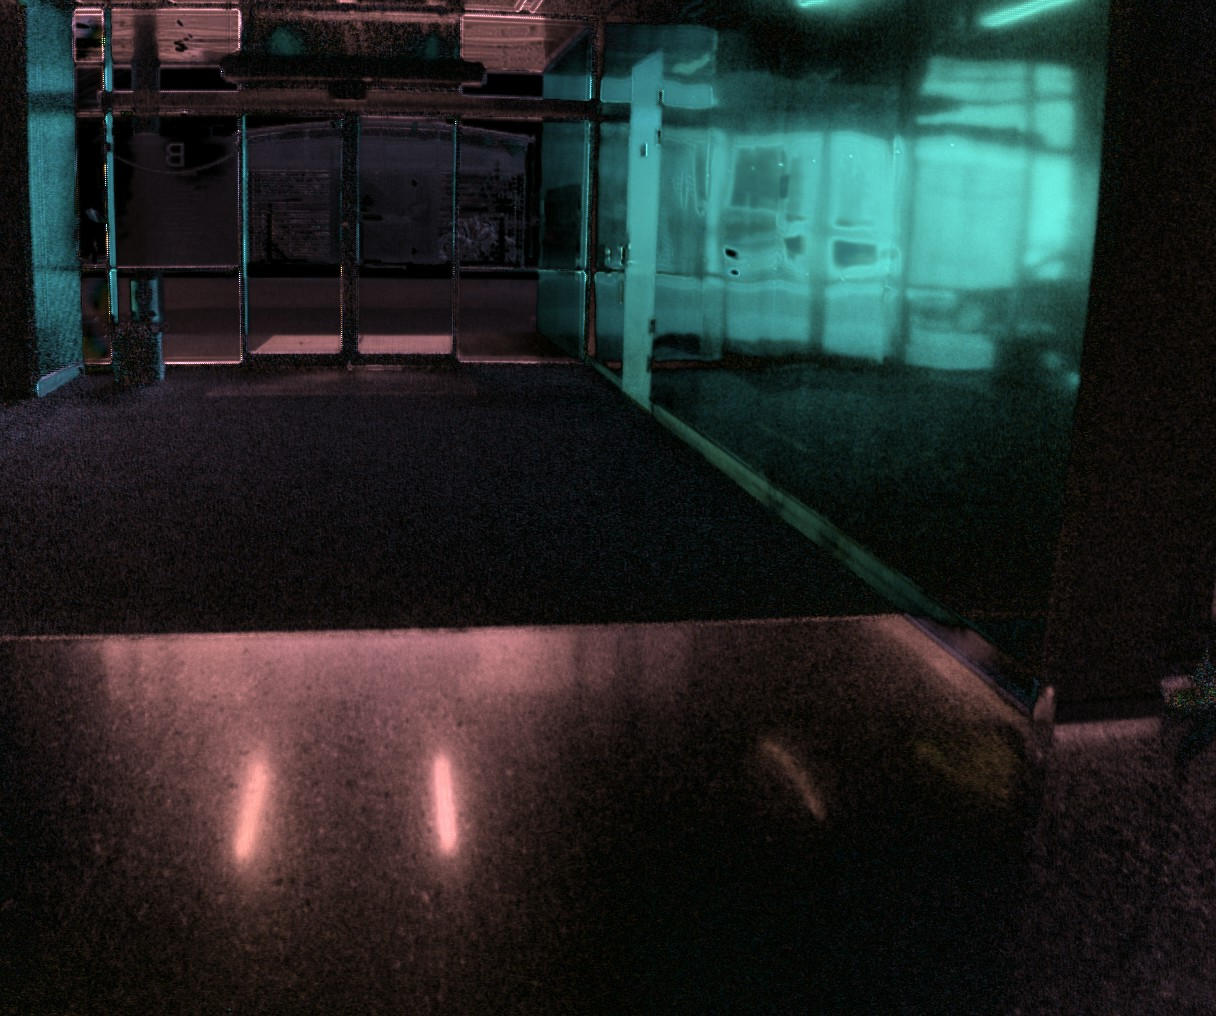
\includegraphics[width=\textwidth]{figures/pictures/img_9306_pol.jpg}
%     \end{subfigure}
%     \caption{High contrast inside environment.}
% \end{figure}
% \vspace{-.5cm}


\begin{figure}[H]
    \begin{subfigure}[T]{.49\textwidth}
        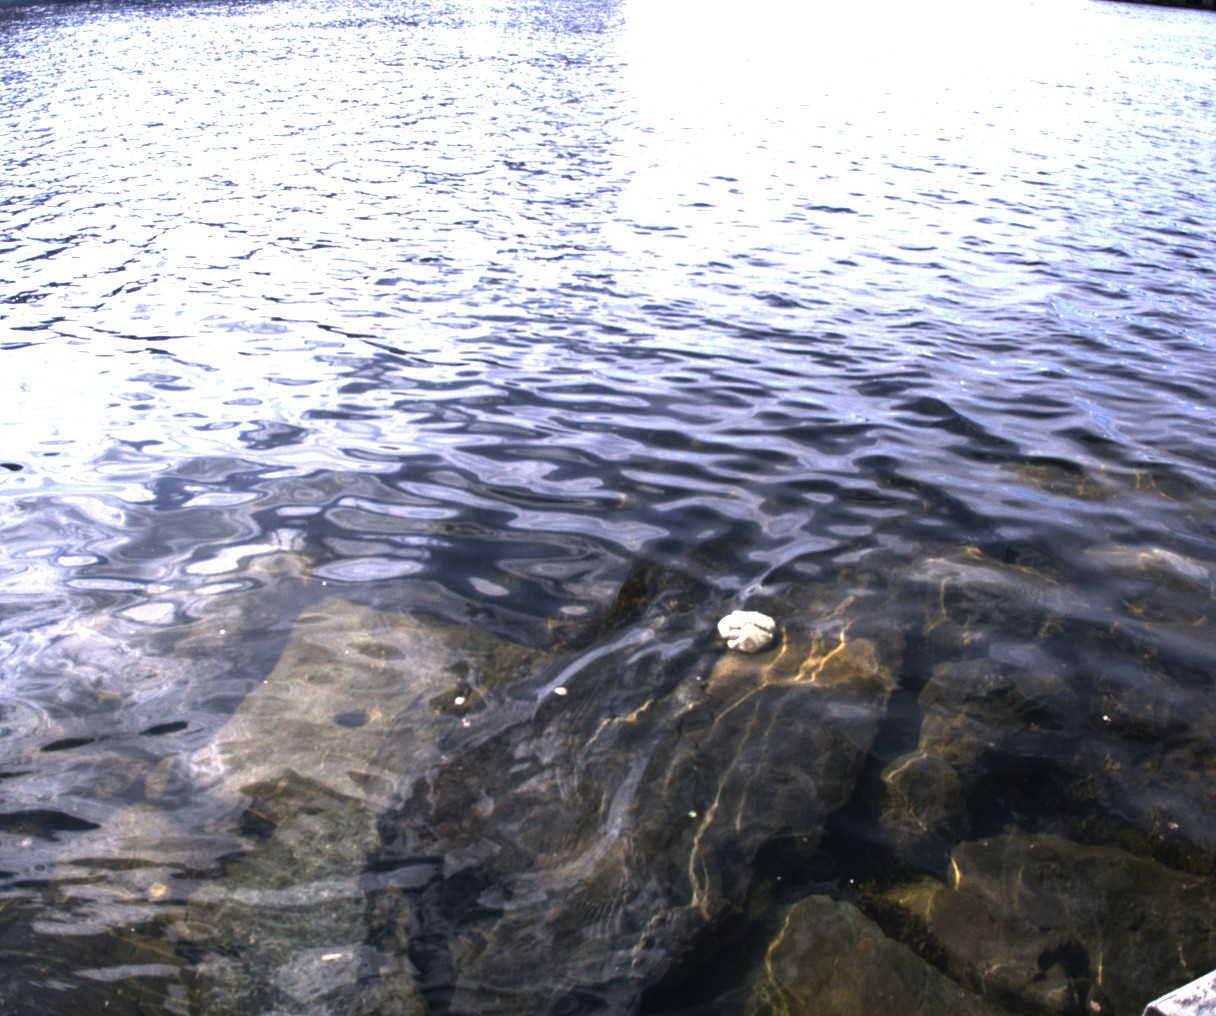
\includegraphics[width=\textwidth]{figures/pictures/img_4722_s0.jpg}
    \end{subfigure} \hfill
    \begin{subfigure}[T]{.49\textwidth}
        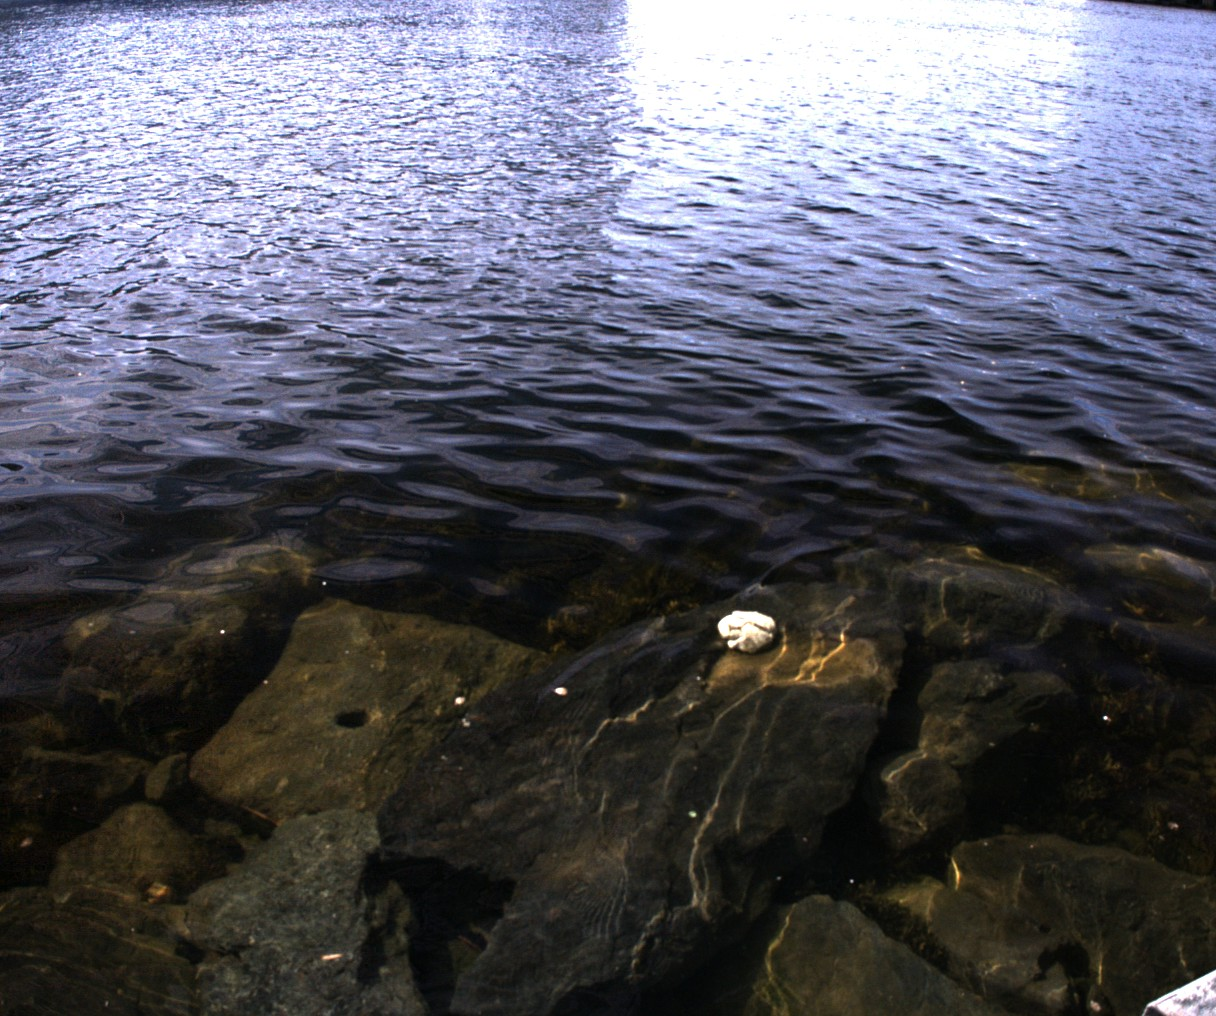
\includegraphics[width=\textwidth]{figures/pictures/img_4722_unpol.jpg}
    \end{subfigure}
    \caption{Image where the linarly polarized light is removed to see whats under the water surface.}
\end{figure}
\vspace{-.5cm}

